\documentclass[manuscript=cmatex]{achemso}
\usepackage[usenames,dvipsnames]{xcolor}
% \definecolor{linkcolor}{RGB}{0,0,240}
\usepackage{listings}
\usepackage{achemso}
\usepackage{makecell}
\usepackage{xr}
\usepackage{appendix}
\usepackage{upgreek}
\usepackage{chemmacros}
\usepackage{siunitx}
\usepackage{textcomp}
\usepackage{natmove}

\definecolor{mygreen}{rgb}{0,0.6,0}
\definecolor{mygray}{rgb}{0.5,0.5,0.5}
\definecolor{mymauve}{rgb}{0.58,0,0.82}

\lstset{ 
  backgroundcolor=\color{white},   % choose the background color; you must add \usepackage{color} or \usepackage{xcolor}; should come as last argument
  basicstyle=\tiny\ttfamily,        % the size of the fonts that are used for the code
  breakatwhitespace=false,         % sets if automatic breaks should only happen at whitespace
  breaklines=true,                 % sets automatic line breaking
  captionpos=b,                    % sets the caption-position to bottom
  commentstyle=\color{mygreen},    % comment style
  deletekeywords={...},            % if you want to delete keywords from the given language
  escapeinside={\%*}{*)},          % if you want to add LaTeX within your code
  extendedchars=true,              % lets you use non-ASCII characters; for 8-bits encodings only, does not work with UTF-8
  firstnumber=1000,                % start line enumeration with line 1000
  frame=single,	                   % adds a frame around the code
  keepspaces=true,                 % keeps spaces in text, useful for keeping indentation of code (possibly needs columns=flexible)
  keywordstyle=\color{blue},       % keyword style
  language=Octave,                 % the language of the code
  morekeywords={*,...},            % if you want to add more keywords to the set
  numbers=left,                    % where to put the line-numbers; possible values are (none, left, right)
  numbersep=5pt,                   % how far the line-numbers are from the code
  numberstyle=\tiny\color{mygray}, % the style that is used for the line-numbers
  rulecolor=\color{black},         % if not set, the frame-color may be changed on line-breaks within not-black text (e.g. comments (green here))
  showspaces=false,                % show spaces everywhere adding particular underscores; it overrides 'showstringspaces'
  showstringspaces=false,          % underline spaces within strings only
  showtabs=false,                  % show tabs within strings adding particular underscores
  stepnumber=2,                    % the step between two line-numbers. If it's 1, each line will be numbered
  stringstyle=\color{mymauve},     % string literal style
  tabsize=2,	                   % sets default tabsize to 2 spaces
  title=\lstname                   % show the filename of files included with \lstinputlisting; also try caption instead of title
}

\captionsetup{font={rm,small}}
\SectionNumbersOn

\usepackage[USenglish]{babel}
\addto\captionsenglish{\renewcommand\chaptername{Section}}
\usepackage{graphicx,array,tabularx,mathtools,siunitx,amsmath,multirow,longtable,float}
\usepackage{hyperref}
\usepackage[nameinlink,noabbrev,capitalize]{cleveref}
\setlength{\footskip}{0.25in}
\usepackage[labelformat=simple]{subfig}
\graphicspath{ {./imgs/} }
\usepackage[labelfont=bf]{caption}
%%%%%%%%%%%%%%%%%%%%%%%%%%%%%%%%%%%%%%%% 
%%%%%%%%%%% 
% \numberwithin{reaction}{section}

\makeatletter
\@ifundefined{ignorespacesafterend}{\def\ignorespacesafterend{\global\@ignoretrue}}{}
\newenvironment{subreactions}{%
  \refstepcounter{reaction}%
  \protected@edef\theparentequation{\thereaction}%
  \setcounter{parentequation}{\value{reaction}}%
  \setcounter{reaction}{0}%
  \def\thereaction{\theparentequation\alph{reaction}}%
  \ignorespaces
}{%
  \setcounter{reaction}{\value{parentequation}}%
  \ignorespacesafterend
}
\externaldocument[main-]{paper}
\makeatother
\title          {Evolution of Copper Surfaces under Plasma Oxidation: Molecular Dynamics Study with Neural Network Potentials}
\author         {Yantao Xia}
\affiliation    {Department of Chemical and Biomolecular Engineering, University of California, Los Angeles, CA 90095, USA}
\email          {xyttyxy@ucla.edu}
\author         {Philippe Sautet}
\affiliation    {Department of Chemical and Biomolecular Engineering, University of California, Los Angeles, CA 90095, USA}
\alsoaffiliation    {Department of Chemistry and Biochemistry, University of California, Los Angeles, CA 90095, USA}
\email          {sautet@ucla.edu}

\makeatletter
\def\@maketitle{%
  \newpage
  \null
  \vskip 2em%
  \begin{center}%
  \let \footnote \thanks
    {\LARGE \@title \par}%
    \vskip 1em%
    {\Large Supplementary Information\par}%
    \vskip 1.5em%
    {\large
      \lineskip .5em%
      \begin{tabular}[t]{c}%
        \@author
      \end{tabular}\par}%
    \vskip 1em%
  \end{center}%
  \par
  \vskip 1.5em}
\makeatother

%%%%%%%%%%%%%%%%%%%%%%%%%%%%%%%%%%%%%%%%%%%%%%%%%%% 
% table formatting commands
\renewcommand{\thesubfigure}{\relax} % no labels on subfigures

\begin{document}
\maketitle
\section{Additional Computational Details}
\subsection{Choice of the exchange-correlation functional}
We estimated the number of required structures to determine whether it is feasible to train a neural network potential at a higher level of theory (e.g. hybrid functionals), following the automatic training method proposed in \cite{schran_automated_2020}. This method estimates the minimum number of structures required to train a neural network potential. The method is outlined as follows:
\begin{enumerate}
\item From a large pool of structures labelled with energies and forces at the PBE level, randomly select 10 structures. 
\item Train two neural network parametrizations \texttt{NNP-1} and \texttt{NNP-2}, differing by their starting point
\item Evaluate energies and forces on all the structures in the dataset, using both potentials.
\item Select the 10 structures where \texttt{NNP-1} and \texttt{NNP-2} disagrees the most in terms of energy, and add to the training set.
\item Retrain both parametrizations. This constitutes as one round of the automated training process. 
\item After each round, the RMSE between \texttt{NNP-1} and \texttt{NNP-2}, between \texttt{NNP-1} and \texttt{DFT}, and between \texttt{NNP-2} and \texttt{DFT} are recorded.
\end{enumerate}
\begin{figure}[h]
  \centering
  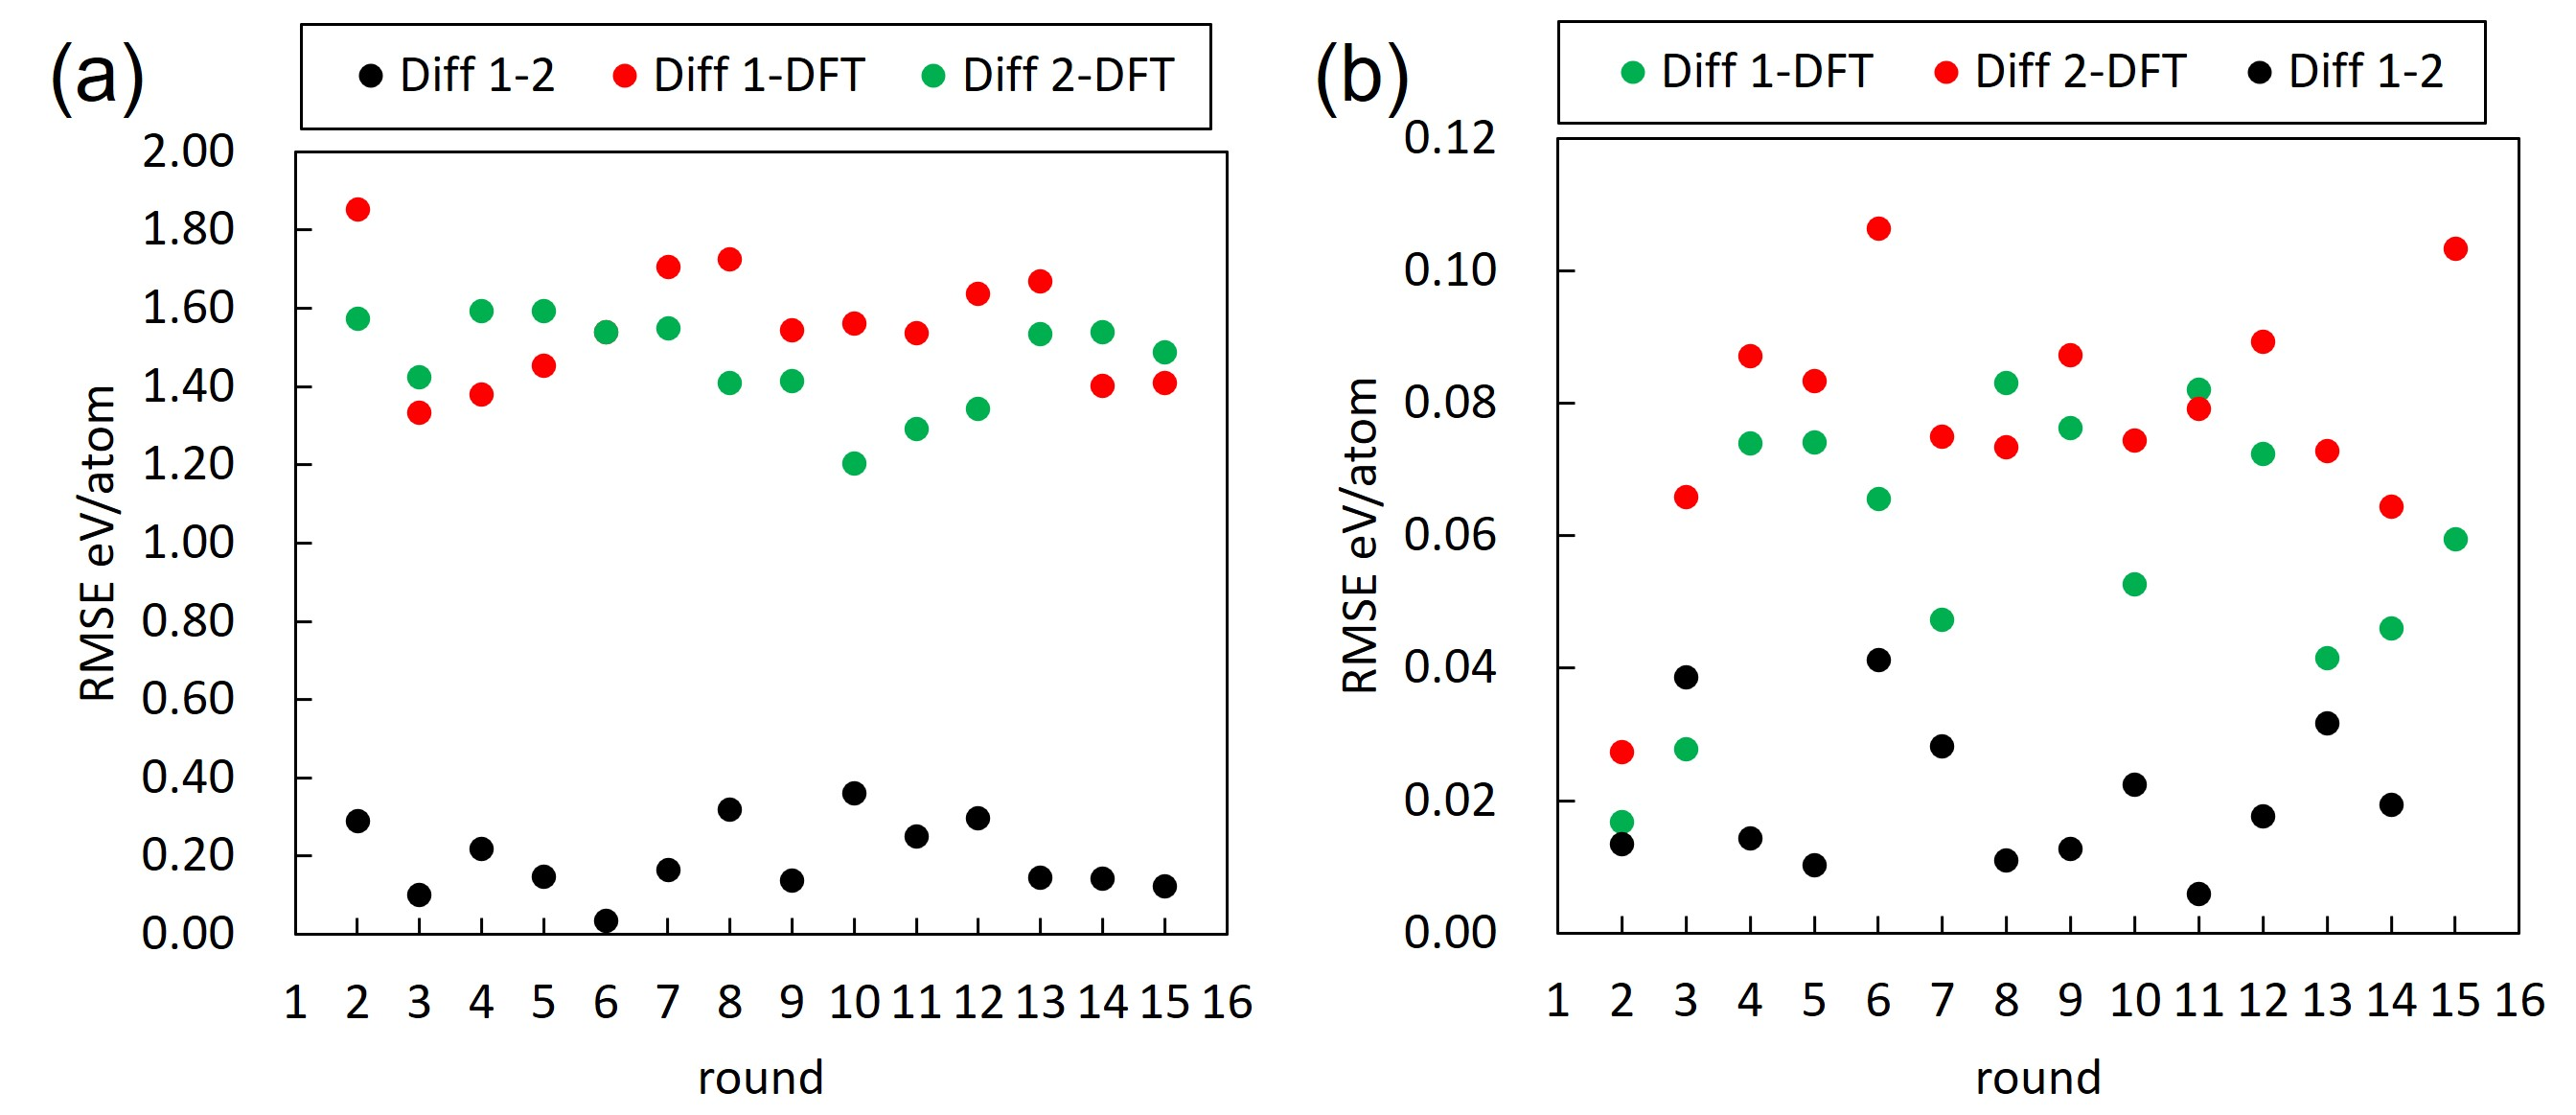
\includegraphics[width=\textwidth]{automated_train}
  \caption[Automated training learning curve]{\textbf{a}: validation errors for the automated training method. ``diff 1-2'' represents the difference between the two network potentials. ``diff 1-DFT'' and ``diff 2-DFT'' represent the difference between the network potentials and the DFT ground truth. All datapoints are evaluated over the whole pool of structures. }
  \label{fig:autotrain}
\end{figure}
\cref{fig:autotrain}a shows that at 150 structures, the validation set error cannot be decreased to a satisfactory value. Note that the unit of the error is in eV per atom as opposed to meV per atom. For all datapoints shown, the error in the training set is less than 5 meV per atom. Training with such a small training data set is prone to overfitting, hence the learning curve is monitored to ensure error on the validation set (the rest of the pool) does not increase with increasing epochs. Since the disagreement between the two networks is much smaller than those between the networks and the ground truth, we clearly do not have enough data in the training set.
Additionally, attempt was made to use the delta learning approach, which has been shown to require a much smaller dataset. The corresponding result is shown in \cref{fig:autotrain}b. To save on computational cost in this proof-of-concept investigation, the network potential is used fit the differences between the PBE and RPBE exchange-correlation functionals, as opposed to a high-level method. Note that the error is decreased by a factor of almost 10 compared with the brute-force fitting to the PBE potential energy surface, indicating that a smaller training set may be used. However, at 150 structures (15 rounds), we do not see a significant decrease in the NNP-DFT difference.
Given the high cost of hybrid functional calculations, a training set much larger than 150 structures cannot be afforded. Therefore, we conclude that from a practical point of view, we can only use the GGA-level of theory. We also note in passing that the exchange-correlation functional must describe properties of both the metal, the molecular and atomic modifier, and the oxide phases accurately. While hybrids could improve the description of the correlated oxide, they in general do not describe the metals well. Hence, the versatile PBE functional is used.
\subsection{Neural network architecture}
The atomic neural networks contains one input layer of 85 nodes (atomic fingerprints), two hidden layers of the 30 nodes each, and one output node for the atomic energy contributions. The fingerprints were chosen to be Behler-Parinello style symmetry functions, with the $\eta$, $r_{s}$, $\lambda$, $\zeta$ parameters generated automatically according to ref. \cite{imbalzano_automatic_2018}. The fingerprints are then ``pruned'' based on the variance of their values across the entire dataset: fingerprints whose value stays constant do not capture the variations in chemical environment and are removed. The n2p2 input file \texttt{input.nn} is given below:
\lstinputlisting{input.nn}
% Additional computational details regarding the architecture of the neural network and the setup of the MD simulations are given in the \textbf{supplementary information}
\subsection{Details regarding data cleaning}
It was found during training, that data cleaning is crucial to the success of training. Due to deficiencies in the early iterations of the network potential, the training MD often leads to unphysical atomic configurations that are few in number but problematic for DFT calculations. These structures cause the DFT calculations to either fail to reach self-consistency or give very high energies. Being few in number, the training routine cannot properly account for them, leading to persistent high errors during training. Therefore, data cleaning is performed to remove 1) configurations with extremely short bond lengths. The cutoff values of the bond length depends on the target kinetic energy, and is determined by the corresponding bond length on \cref{main-fig:val_close}. Additionally, in the very early stages, clearly impossible structures with lost \ch{Cu} atoms, disintegrated slabs, etc. are removed. 
\subsection{Additional training and model validation information}
\subsubsection{Re-parametrization of the ReaxFF starting point}
The starting point of the parametrization was taken to be the ReaxFF potential. Since original training set does not include short-distance interactions of Cu/O, the as-found potential is not very stable to plasma impact even at a kinetic energy of 5 eV. As a result, the inner wall repulsion term, implemented in ReaxFF, was re-parametrized to the potential energy curves of \ch{Cu}-\ch{Cu}, \ch{Cu}-\ch{O}, and \ch{O}-\ch{O} dimers, calculated at the PBE level. The comparison of refitted \ch{O2} diatomic molecular potential energy surface is compared with DFT values in \cref{fig:o4}. This step ensures the exponetntial inner wall repulsion is reproduced. 
\begin{figure}[h]
  \centering
  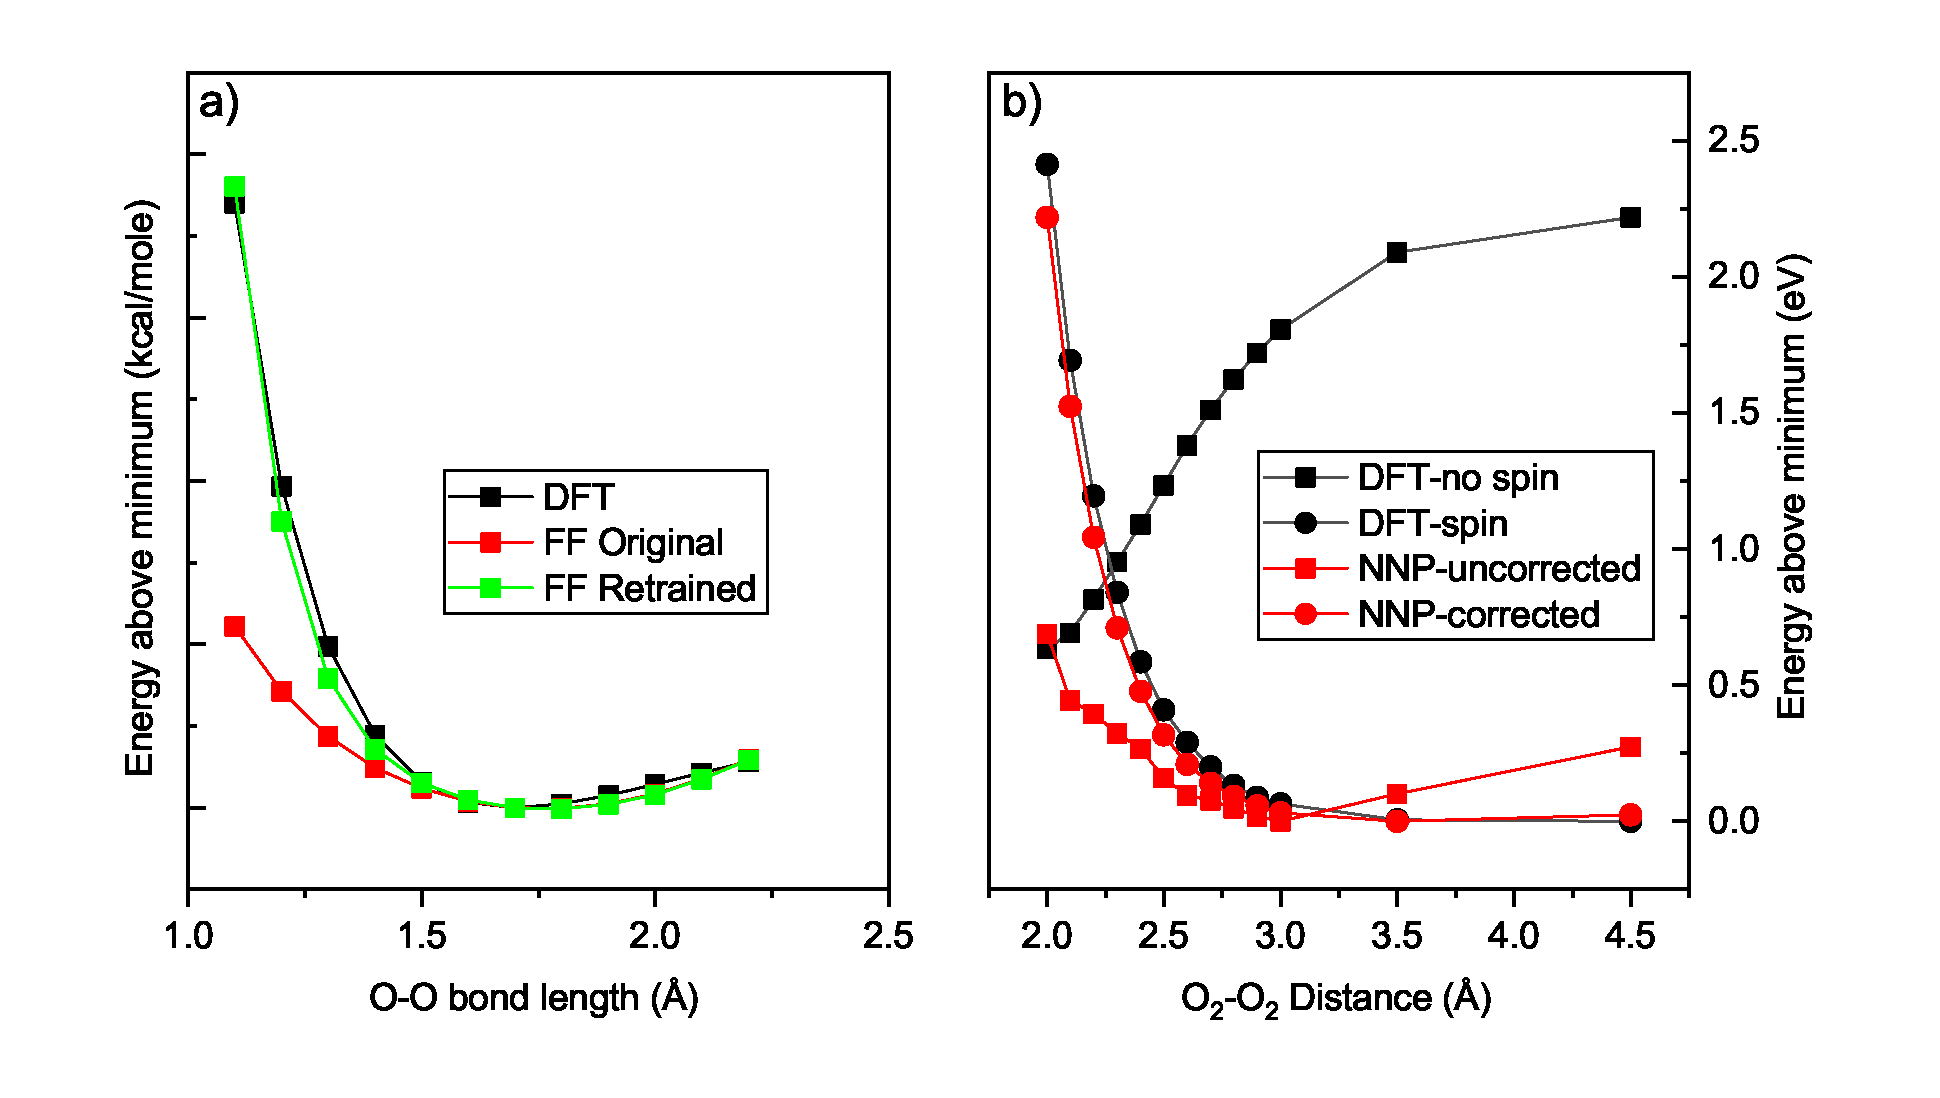
\includegraphics[width=\textwidth]{o2o4}
  \caption[PES of \ch{O2}-\ch{O2} interaction using DFT and NNP]{\textbf{(a)}: comparison of potential energy of an \ch{O2} molecule using literature ReaxFF parameter set (FF original), reparametrized ReaxFF parameter set (FF-retrained), and DFT. \textbf{(b)}: comparison of the potential energy surface two shoulder-to-shoulder \ch{O2} molecules, using spin unpolarized DFT(DFT-no spin), spin polarized DFT (DFT-spin), and two parameter sets of the neural network potential before and after correcting for oxygen clustering.}
  \label{fig:o4}
\end{figure}
\subsubsection{Collision event tracking in training}
While the addition rate of ions is fixed at one per 10000 steps, the ions are added at varying heights and the surface is not smooth. Therefore, to sample short-distance structures efficiently, an analysis program tracks the minimal distance between the O atoms and Cu atoms at each time step in the trajectory. This signal is inverted and peak analysis is performed. The peaks are treated as steps where collision events occured and the steps near the peaks are sampled at regular spacing. A collection of scripts for dataset generation and data analysis scripts used in this study are available at \href{http://github.com/xyttyxy/ale_scripts}{GitHub}.

\subsubsection{Details of training iterations}
The training routines were able to minimize the energy and force errors on the test set to \SI{2.32}{meV / atom} and $\SI{0.15}{eV/\angstrom}$, respectively. The new neural network parametrization, termed \textbf{nnp1}, was used in identical MD impact simulations as those used to generate \textbf{md0}, to generate a new set of snapshots. In subsequent steps, the ReaxFF force field itself, and the ReaxFF-based \textbf{md0} dataset, were not used. Again, 25 distinct MD runs were performed. After a cleaning procedure identical to that applied to \textbf{md0}, yielding \textbf{md1} dataset, containing 2716 structures. Before training was performed on this new dataset, the self-consistency of the neural network potential \textbf{nnp1} was tested by calculating its prediction error on the dataset obtained via MD driven by itself (\textbf{md1}), as an benchmark for the out-of-sample error. Not surprisingly, the energy error is \SI{88.67}{meV / atom} and the force error is $\SI{1.98}{eV/\angstrom}$. The fact that the out-of-sample error is almost two orders of magnitude higher than the in-sample error is used as an indication that the sample (ReaxFF-generated at this stage) has a different underlying ``distritbuion'' than the ground truth (in this case, the DFT potential energy surface), in accordance with statistical learning theory. Therefore, the neural network potential is retrained on the dataset composed of \textbf{md1}, to yield a test set error \SI{3.14}{meV / atom} and $\SI{0.17}{eV/\angstrom}$, respectively on energies and forces. New MD structures were generated (\textbf{md2}), and again the out-of-sample prediction error is calculated to be \SI{2.78}{meV / atom} and $\SI{0.13}{eV/\angstrom}$, respectively. This indicates that the neural network potential, within the MD setup used to generate the training configurations, does not extrapolate. As a finishing step, \textbf{md1} and \textbf{md2} are combined to retrain the neural network potential, yielding \textbf{nnp2}. 

The \textbf{nnp2} potential, however, was only trained on a $(3\times3)$ Cu (100) cell with 5 layers. To avoid artifacts introduced by periodic boundary conditions, the production simulations needs to be run on much larger cells. Attempting to do so, however, creates extrapolation problem. Two reasons are underlying. The first is that in the small cell used for training, the lateral dimensions were shorter than the cutoff length of the neural network potential. When the oxygen molecule dissociates, the individual atoms is always inside the cutoff spheres of each other, preventing the chemical environment of isolated oxygen atom on the copper slab from being included in the training set. The second reason is the thickness of the slab is less than twice the cutoff radius. Therefore, even the central \ch{Cu} atom is not completely surrounded by other \ch{Cu} atoms, preventing the bulk copper environment from being described accurately. A parallel problem of not able to describe bulk oxide manifests itself when the oxide thickness approaches $2r_c$. As the choice of a $(3\times3\times5)$ slab model was to keep the cost of dataset preparation low, these problems were remedied by supplementary datasets of 1) single O atom impact simulations, concentrated on describing the very first impacting event (\textbf{impact\_initial}, 604 configurations), 2) thick $(3\times3\times8)$ \ch{Cu} and oxide slabs, produced by running impact simulations at elevated temperatures until the entire slab is oxidized (\textbf{thick}, 256 configurations). 3) snapshots of high temperature equilibrium MD of bulk \ch{CuO} and \ch{Cu2O} supercells (\textbf{bulk}, 300 configurations). After these supplemental configurations were added to the dataset, the retrained NNP was able to sustain simulations upto 1 nanosecond on a $(20\times20\times10)$ slab with 4000 atoms. Simulations on larger slabs are feasible but not attempted.
% The structures are illustrated in \textbf{SI}
\begin{figure}[h]
  \centering
  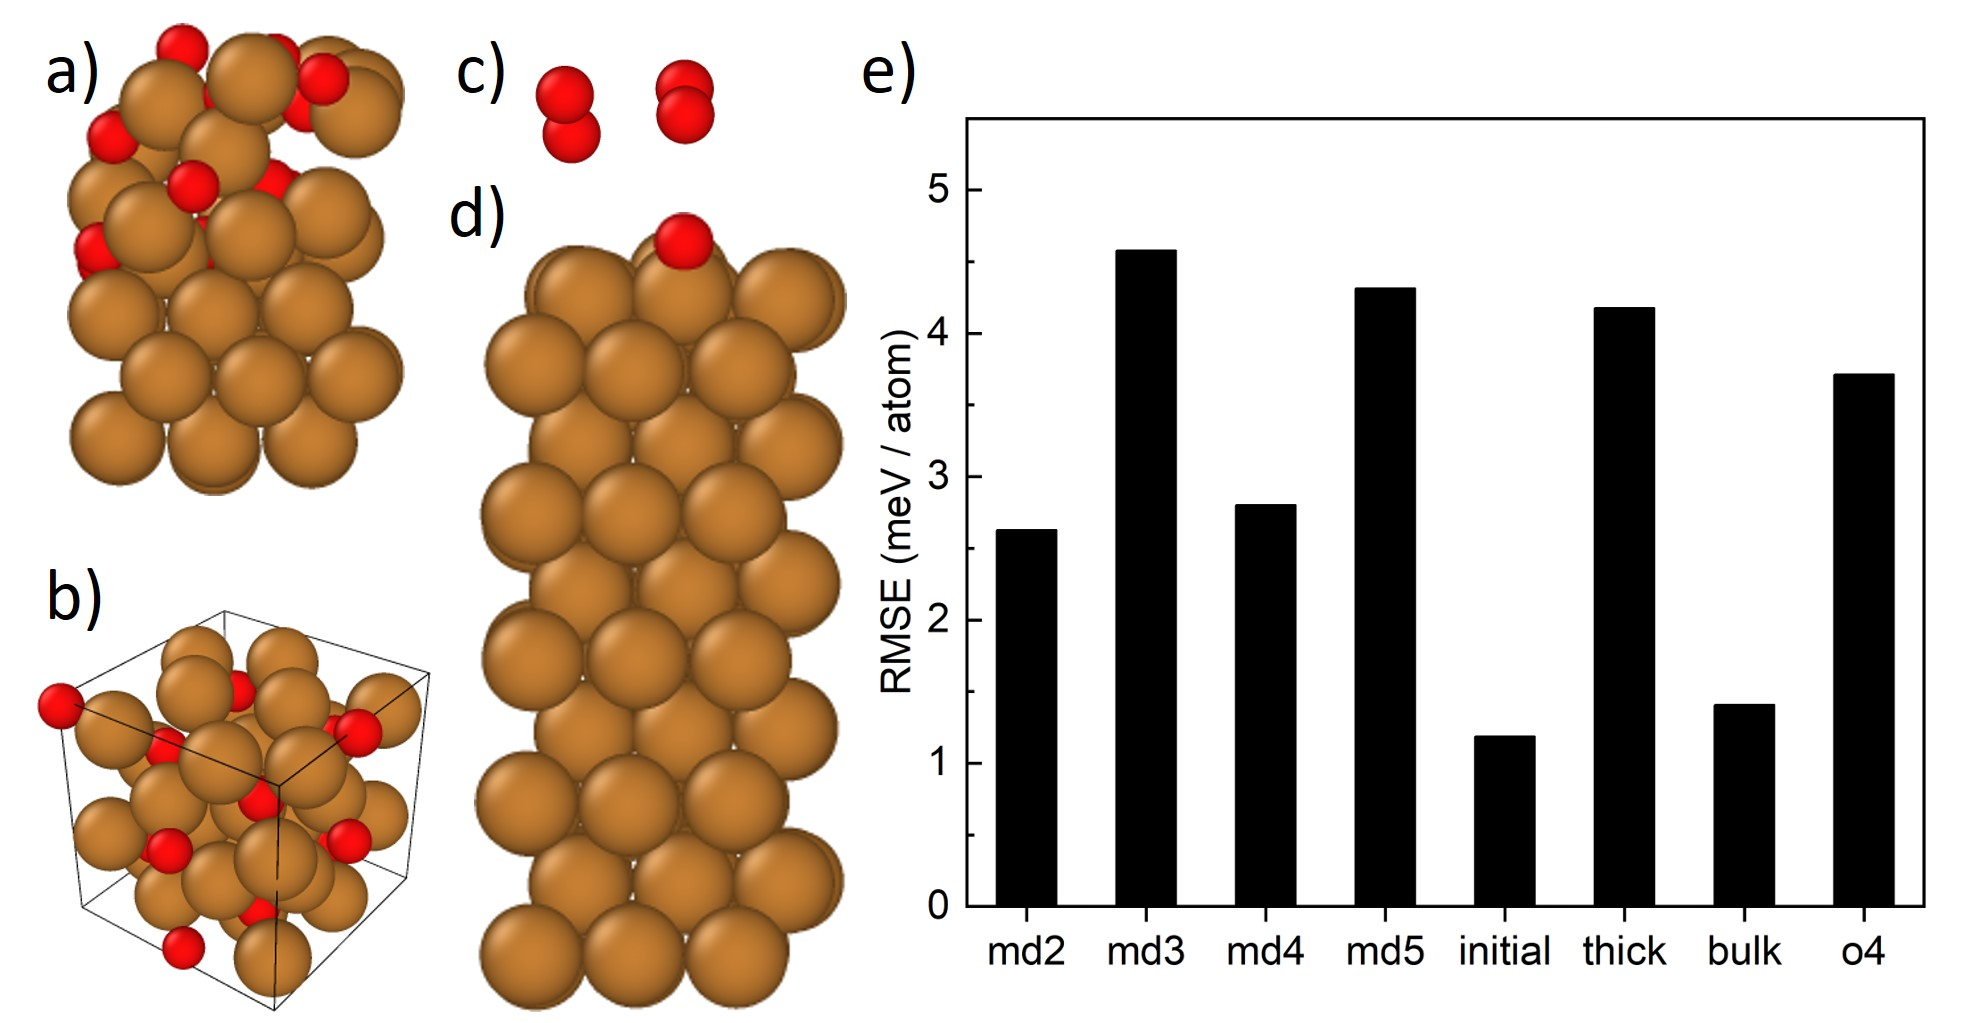
\includegraphics[width=\textwidth]{structures}
  \caption[Representative structures used in training and energy error on the subsets]{\textbf{(a)-(d)}: structures used in training: \textbf{(a)}: snapshots of \ch{Cu} (100) slab under oxygen bombardment MD, this comprises the majority of the dataset; \textbf{(b)}: bulk copper oxide structure; \textbf{(c)}: \ch{O2}-\ch{O2} interaction for oxygen clustering correction calculated by enforcing high-spin state; \textbf{(d)}: thick slab structures to minimize extrapolation error. \textbf{(e)}: errors on each subdivision of the dataset showing the potential performs well on all relevant environments.}
  \label{fig:subset}
\end{figure}
\section{Post-processing and analysis of MD trajectories}
\subsection{Calculation of oxide film thickness}
The film thicknesses calculation involves the following steps:
\begin{enumerate}
\item locating the top surface by identifying the interfacial atoms. This is done using the pytim module, with the method described in \cite{partay_new_2008}. 
\item The bottom surface is located in a similar fashion. However, the method cannot be used to determine interfacial atoms where the density stays more or less constant but the composition changes abruptly. Therefore, all the copper atoms were removed prior to detecting the interfacial oxygen atoms. 
\item The average $z$-coordinate of the atoms in the top and bottom surface are calculated, and the difference $\delta z = \bar{z}_{\mathrm{top}}-\bar{z}_{\mathrm{bottom}}$ is reported as the film thickness. In very thin films the top and bottom surface atoms overlap, and thickness is rounded up to 0. 
\end{enumerate}
\subsection{Comparison of simulated and experimental impact rates}
Given the pressure of the plasma processing step, the impact frequency can be calculated using the kinetic theory of gases:
\begin{equation*}
  J_{\mathrm{collision}} = \frac{P}{\sqrt{2\pi m k_BT}}
\end{equation*}
At a pressure of \SI{30}{mTorr}, $J_{\mathrm{collision}}=4.378\times 10^{-10} \mathrm{\frac{1}{nm^2 fs}}$. The slab used during production MD had \SI{6.3}{nm^2} area, corresponding to an impact frequency of \SI{8.71e-10}{fs}. Therefore, to capture even one impact event at laboratory time scale, we need \SI{1.15e3}{ns}, clearly beyond current capabilities. Therefore, at best, the MD simulations of plasma processing may be related to laboratory times via fluences of the ions.
\subsection{Characterization of oxide composition}
To determine the chemical composition of the oxide film, we analyzed the local environment of each atom using bond orientational order parameters.\cite{steinhardt_bond-orientational_1983} The voronoi tesellation averaged version, shown below, is used.\cite{mickel_shortcomings_2013}
\begin{equation*}
  q'_l(a) = \sqrt{\frac{4\pi}{2l+1}\sum_{m=-l}^{l}|\frac{A(f)}{A}\sum_{b\in \mathrm{NN}(a)}Y_{lm}(\theta_{ab}, \psi_{ab})|^2}
\end{equation*}
, where $Y_{lm}$ is a spherical harmonic function of degree $l$ and order $m$, $\theta_{ab}$ and $\psi_{ab}$ are polar and azimuthal angles of the distance vector between neighboring atoms in spherical coordinates, $A(f)$ and $A$ are the separating surface in the voronoi tesselation between neighboring atoms and the total area of the voronoi cell of the center atom, respectively. 
\subsection{Tracing the range of thermal agitations}
To study the thermal activation of diffusion inside the oxide, the diffusivities at various temperatures are calculated (see details in \textbf{SI}). Starting with the detection of the collision event detailed above, the atoms near the impact site are monitored for their velocties. The atom with velocities exceeding the cutoff velocity is added to the tracked hot atoms. The algorithm is repeated recursively in the list of ``hot atoms'' for each time step, therefore accounting for all the atoms affected by the thermal agitation. The cutoff velocity is a parameter specified in terms of the probability of particles with such velocities being present in the integrated Maxwell-Boltzmann distribution, which the velocity distributions in a amorphous solid are assumed to have.\cite{mohazzabi_maxwell-boltzmann_2018}. In this work, this cutoff probability is $1\times 10^{-5}$
\subsection{Fitting of the oxide thickness growth rate}
Temperature distributions in the film clearly depends on the kinetic energy of the impact ions, the atomic configurations of the slab, and the thickness. The subject slab is taken at the end of the long-time MD with the $T_s=\SI{353}{K}$, $E_K=\SI{20}{eV}$, $\mathrm{n2i}=20$, because this structure reached the greatest thickness. The structure was re-equilibrated at \SI{353}{K} for a long time to desorb all the physisorbed \ch{O2} molecules. In calculating the temperature response of the oxide slab to ion impact, a single ion was launched at the surface at 500 different random positions above the slab, and the trajectory is followed in NVE ensemble for 10000 steps, corresponding to roughly \SI{4}{ps}. Two sets of simulations were performed with $E_k=\SI{10}{eV}$ and $E_k=\SI{20}{eV}$. The oxide region in the resulting trajectories (500 for one $E_K$) was divided into 20 layers in the $z$-direction, and the distributions of atomic kinetic energy were calculated and converted to the distribution of ``atomic temperatures'' based on the equipartition principle. 
\clearpage

\bibliography{ref}

\end{document}

